Tο καθιερωμένο πρότυπο 
%της σωματιδιακής φυσικής τα σωματίδια ύλης και τα μποζόνια %βαθμίδας υπόκεινται στο μηχανισμό αυθόρμητης ρήξης της %συμμετρίας. Το πρότυπο 
βασίζεται στη θεωρία των Glashow, Weinberg και Salam, η οποία ενοποιεί τις ηλεκτρομγνητικές και τις ασθενείς αλληλεπιδράσεις %(ηλεκτρασθενής θεωρία) 
σε μια συμμετρική, μη-αβελιανή θεωρία βαθμίδας $SU(2)\subscr{L}\times U(1)\subscr{Y}$. Η ηλεκτρασθεής συμμετρία αυτή σπάζει αυθόρμητα (μηχανισμός Higgs) με σημαντικές φυσικές συνέπειες \cite{Peskin:1995ev}. Στο κεφάλαιο αυτό παρουσιάζουμε μερικές από τις συνέπειες αυτές, και τις επανεξετάζουμε στην περίπτωση ισχυρών μαγνητικών πεδίων υποβάθρου. Μία τέτοια κατάσταση εμφανίζεται στην εξωτερική περιοχή του ορίζοντα μιας μαγνητικά φορτισμένης μελανής οπής. 

\section{Αυθόρμητη ρήξη συμμετρίας}\label{spontaneous symmetry breaking}
Οι συμμετρίες ενός φυσικού μοντέλου είναι μετσχηματισμοί που αφήνουν αμετάβλητες παρατηρήσιμες φυσικές ποσότητες, όπως η ενέργεια. 
%των καταστάσεων του  αναφερόμαστε στην αμεταβλητότητα των %φυσικών ποσοτήτων ως προς μετασχηματισμούς των κβαντικών %καταστάσεων. 
Οι μετασχηματισμοί αναπαρίστανται ως εκθετικοί μοναδιακοί τελεστές $U=e\superscr{iT\superscr{i}\theta\superscr{i}}$ που δρουν στο χώρο Hilbert, $\mathcal{H}$, των κβαντικών καταστάσεων
\begin{equation}
    U:\mathcal{H}\rightarrow\mathcal{H}
\end{equation}
όπου $T^i$ οι ερμιτιανοί γεννήτορες των μετασχηματισμών (με τις απαραίτητες μεταθετικές ιδιότητες). Οι μοναδιακοί τελεστές δρουν γραμμικά στις κβαντικές καταστάσεις, οι οποίες 
%δρα σε συγκεκριμένους βαθμούς ελευθερίας των κβαντικών πεδίων %τα οποία, 
στη γενικότερη περίπτωση μεταβάλλονται
\begin{equation}\label{transformation of psi under the group of unitary operators}
    \left|\psi\right>\mapsto\left|\psi '\right>\equiv U\left|\psi\right> = e\superscr{iT\superscr{i}\theta\superscr{i}}\left|\psi\right> \qquad  \left|\psi\right>\ne \left|\psi'\right>
\end{equation}
Αντίθετα, εάν μια κατάσταση $ \left|\psi\right>$ παραμένει αναλλοίωτη, τότε είναι συμμετρική ως προς τους μετασχηματισμούς. Σε αυτή τη περίπτωση η $ \left|\psi\right>$ είναι ιδιοκατάσταση του τελεστή $U$ και καταστρέφεται από τους αντίστοιχους γεννήτορες
\begin{equation}\label{psi is symmetric under the unitary transformation of the group}
    \left|\psi\right>\mapsto U \left|\psi\right> = \left|\psi\right>, \qquad T\superscr{i} \left|\psi\right>=0
\end{equation}
%Η αλλοίωση όμως των κβαντικών καταστάσεων δεν μεταφέρεται κατ' %ανάγκη στη χαμιλτονιανή του φυσικού μοντέλου. 
\\

Οι μετασχηματισμοί λοιπόν που αφήνουν τη χαμιλτονιανή αναλλοίωτη αποτελούν συμμετρίες της θεωρίας. Οι αντίστοιχοι μοναδιακοί τελεστές και οι γεννήτορες τους μετατίθενται με τη χαμιλτονιανή
\begin{equation}\label{commutator with hamiltonian for a symmetry}
    [H,U]=[H,T\superscr{a}]=0
\end{equation}
%Είναι σημαντικό να σημειωθεί ότι η \eqref{commutator with %hamiltonian for a symmetry} ισχύει ανεξάρτητα του αν η %κατάσταση του συστήματος $\left|\psi\right>$ αλλοιώνεται από το %μετασχηματισμό \eqref{transformation of psi under the group of %unitary operators} ή όχι \eqref{psi is symmetric under the %unitary transformation of the group}. 
\\

Εκδηλώνονται σημαντικά φαινόμενα όταν η δράση των μετασχηματισμών συμμετρίας μεταβάλλουν τη βασική κατάσταση του συστήματος, ή την κατάσταση κενού σε ένα σύστημα κβαντικού πεδίου $\left|\,\Omega\right>$ 
%που ορίζεται ως η κατάσταση μηδενικής τετραορμής %$P\superscr{\mu}=(H,\vec{P})$ 
%\begin{equation}\label{vacuum state zero momentum}
%    P\superscr{\mu}\left|\,\Omega\right>=0\qquad\vec{P}\left|\,%\Omega\right>=0 
%\end{equation}
Η $\left|\,\Omega\subscr{i}\right>$ μετασχηματίζεται σε μια ορθογώνια κατάσταση $\left|\Omega\subscr{j}\right>$, σύμφωνα με την \eqref{transformation of psi under the group of unitary operators} 
\begin{equation}\label{transformation of vacuum state}
    \left|\,\Omega\subscr{i}\right> \mapsto \left|\Omega\subscr{j}\right> \equiv U\left|\,\Omega\subscr{i}\right>\ne \left|\,\Omega\subscr{i}\right> \qquad \left<\Omega\subscr{i}\,|\,\Omega\subscr{j}\right>=\de\subscr{ij}
\end{equation}
%γεγονός που την καθιστά μη συμμετρική ως προς τους %μετασχηματισμούς. 
Με χρήση του μεταθέτη \eqref{commutator with hamiltonian for a symmetry} είναι φανερό ότι η νέα κατάσταση $\left|\,\Omega'\right>$ είναι επίσης ιδιοκατάσταση της χαμιλτονιανής με την ίδια ιδιοτιμή 
\begin{equation}
    [H,U]\left|\,\Omega\right>=0\Rightarrow H(U\left|\,\Omega\right>)=UH\left|\,\Omega\right>=E\subscr{\Omega}U\left|\,\Omega\right>
\end{equation}
Οι εκφυλισμένες καταστάσεις έχουν την ίδια ενέργεια $E\subscr{\Omega}$ αλλά διαφορετικές αναμενόμενες τιμές για διάφορους άλλους τελεστές. Μια υπέρθεση όλων αυτών των καταστάσεων, όπως προβλέπεται στη μη σχετικιστική κβαντική μηχανική, σέβεται την συμμετρία και αίρει τον εκφυλισμό. 
Όπως δείχνουμε στη συνέχεια, η πραγματική βασική κατάσταση στην περίπτωση ενός κβαντομηχανικού μοντέλου δεν είναι κάποια από τις καταστάσεις που ελαχιστοποιούν τη δυναμική ενέργεια, αλλά μια συμμετρική υπέρθεση τους. Αντίθετα, στην κβαντική θεωρία πεδίων, οι βασικές καταστάσεις μπορεί να σπάζουν τη συμμτερία 
%να είναι μια από τις εκφυλισμένες καταστάσεις, η οποία όμως %είναι ευαίσθητη στους μετασχηματισμούς της ομάδας συμμετρίας 
σύμφωνα με την \eqref{transformation of vacuum state}. Όταν συμβαίνει αυτό θα λέμε ότι η συμμετρία σπάζει αυθόρμητα.

\subsection{Κβαντομηχανικό παράδειγμα}
Ως πρώτο παράδειγμα, ας θεωρήσουμε ένα μη σχετικιστικό κβαντικό σωματίδιο μάζας $m$ το οποίο κινείται σε μία διάσταση υπό την επίδραση δύναμης που απορρέει από το δυναμικό 
%και συνάρτηση πυκνότητας πιθανότητας $\psi(x)$ εντός του δυναμικού 
$V(x)= \frac{1}{2}m\omega\superscr{2}x\superscr{2}(x\superscr{2}-1)$. Η χαμιλτονιανή του συστήματος παραμένει αναλλοίωτη ως προς τη συμμτερία ομοτιμάς $x \to -x$, που είναι μια διακριτή $\mathbb{Z}\subscr{2}$ συμμετρία. Το δυναμικό έχει δύο ελάχιστα %σημεία ευσταθούς ισορροπίας 
για $x=a,-a$. Εκδηλώνει μέγιστο στη θέση $x=0$. Ένα κλασικό σωματίδιο με συνολική ενέργεια $E<V(0)$ είναι εξαναγκασμένο να εκτελεί ταλαντώσεις γύρω από ένα ελάχιστο, χωρίς να μπορεί να διέλθει του φράγματος δυναμικού. Αυτό όμως, δεν συμβαίνει στο κβαντικό επίπεδο εξαιτίας του φαινομένου της σήραγγας. Στο χώρο Hilbert, οι δύο εκφυλισμένες καταστάσεις είναι οι $\left|a\right>$ και $\left|-a\right>$ με την κάθε μια να επικεντρώνεται γύρω από την αντίστοιχη κλασική θέση ισορροπίας 
\begin{equation}
    \left<-a\right|\hat{x}\left|-a\right>=-a\qquad\left<a\right|\hat{x}\left|a\right>=a
\end{equation}
Οι δύο αυές καταστάσεις δεν περιγράφουν τη βασική κατάσταση του συστήματος, αφού το κβαντικό σωματίδιο μπορεί να διέλθει του φράγματος με μη μηδενική πιθανότητα, η οποία υπολογίζεται στην προσέγγιση WKB (π.χ. \cite{griffiths_qm})
\begin{equation}
    T=\exp\left[ -\frac{2}{\hbar}\int_{-a}^{a}dx\,[2m(V-E)]\superscr{1/2} \right]
\end{equation}
Η χαμιλτονιανή έχει τα εξής πινακοστοιχεία μεταξύ των δύο εκφυλισμένων καταστάσεων $\left|a\right>$ και $\left|-a\right>$: 
\begin{equation}
\begin{split}
    &\left<-a\right|\hat{H}\left|-a\right>=\left<a\right|\hat{H}\left|a\right>=\frac{1}{2}\hbar\omega\\
    &\left<-a\right|\hat{H}\left|a\right>=\left<a\right|\hat{H}\left|-a\right>=\frac{\hbar\omega}{2\pi}e\superscr{-m\omega a\superscr{2}/\hbar}
\end{split}
\end{equation}
Η βασική κατάσταση αποτελεί γραμμικό συνδυασμό των $\left|a\right>$ και $\left|-a\right>$. Πράγματι, ο εκφυλισμός αίρεται και η κατάσταση χαμηλότερης ενέργειας είναι ο συμμετρικός συνδυασμός $\left|S\right>$, με ενέργεια $E\subscr{\text{S}}$ που δίδεται από την έκφραση
\begin{equation}
    \left|S\right>=\frac{\left|a\right>+\left|-a\right>}{\sqrt{2}}\qquad E\subscr{S}=\frac{1}{2}\hbar\omega-\frac{\hbar\omega}{2\pi}e\superscr{-m\omega a\superscr{2}/\hbar}
\end{equation}
Η αναμενόμενη τιμή του τελεστή θέσης $\hat{x}$ στη βασική κατάσταση είναι επομένως αμετάβλητη ως κατοπτρικούς  μετασχηματισμούς ομοτιμίας, εξαιτίας της αναλλοιότητας της βασικής κατάστασης
\begin{equation}
    \left<S\right| \hat{x} \left|S\right>\,=\,0
\end{equation}

\subsection{Συνεχείς συμμετρίες και μποζόνια Goldstone}
Στη κβαντική θεωρία πεδίων, όταν σπάσουν αυθόρμητα συνεχείς καθολικές συμμετρίες 
%ομάδων Lie μπορούν να σπάσουν οδηγώντας σε ενδιαφέροντα %φαινόμενα. Η ρήξη καθολικών (global) συμμετριών συνοδεύεται από
εμφανίζονται άμαζα σωματίδια στο φάσμα, τα σωματίδια Goldstone, σύμφωνα με το θεώρημα Goldstone. Στην περίπτωση τοπικών  συμμετριών, οι καταστάσεις Goldstone συνδυάζονται με τα μποζόνια βαθμίδας για να δώσουν ένα σωματίδιο με σπιν $1$ και μη μηδενική μάζα \cite{Peskin:1995ev}.  
%που έχουν εισαχθεί για την αναλλοίωτη ως προς βαθμίδα %λειτουργία της θεωρίας. Είναι ενδιαφέρον ότι 
Tο αυθόρμητο
σπάσιμο συμμετρίας δεν εκδηλώνεται σε χωροχρόνους με δύο ή λιγότερες διαστάσεις λόγω των ισχυρών κβαντικών διακυμάνσεων των μποζονίων Goldstone. 
%σε αυτές τις διαστάσεις - απόδειξη του Sidney Coleman. 

\subsection{Κατάσταση κενού στην κβαντική θεωρία πεδίου}
Σε μια κβαντική θεωρία πεδίου, ενδέχεται οι καταστάσεις που ελαχιστοποιούν την ενέργεια να είναι εκφυλισμένες. Οι καταστάσεις αυτές μετασχηματίζονται η μια στην άλλη μέσω συμμετριών, όπως αναφέραμε προηγουμένως, και χαρακτηρίζονται από μη μηδενικές τιμές κάποιου πεδιακού τελεστή.
%Βάση όμως της αρχής cluster decomposition 
Στις τέσσερις διαστάσεις, είναι δυνατό το σύστημα να βρεθεί σε 
%περιοριστεί σε μόνο 
μία από τις εκφυλισμένες καταστάσεις αυτές, η οποία όμως δεν είναι αμετάβλητη, 
%καθιστώντας την κατάσταση κενού μη συμμετρική - 
οδηγώντας σε αυθόρμητο σπάσιμο της συμμετρίας. Αυτό μπορεί να δειχθεί εφαρμόζοντας την αρχή της ανάλυσης κατά κλάστερς \cite{weinberg_1996}.
Με βάση την αρχή αυτή τα αποτελέσματα πειραμάτων  
%αφορά την επιβολή της φυσικής προϋπόθεσης ότι, πειράματα 
σε περιοχές 
%απόμακρα σημεία 
του χώρου που απέχουν κατά πολύ μεγάλη απόσταση, δηλαδή για $\mathbf{x}\equiv \Vec{x}$, $\mathbf{\text{\textbf{y}}}\equiv \Vec{\text{y}}$, $|\mathbf{x}-\text{\textbf{y}}|\rightarrow\infty$, είναι ανεξάρτητα μεταξύ τους. Συνεπώς, στην πραγματική κατάσταση κενού, $\left|\text{VAC}\right>$, η αναμενόμενη τιμή γινομένου δύο πεδιακών τελεστών, σε δύο σημεία των περιοχών αυτών αντίστοιχα, παραγοντοποιείται σε γινόμενο των αναμενόμενων τιμών του κάθε τελεστή ξεχωριστά \cite{weinberg_1996}
\begin{equation}
    \lim\subscr{|\mathbf{x}-\text{\textbf{y}}|\rightarrow\infty}\left<\text{VAC}\right|A(\mathbf{x})B(\text{\textbf{y}})\left|\text{VAC}\right>=\left<\text{VAC}\right|A(\mathbf{x})\left|\text{VAC}\right>\left<\text{VAC}\right|B(\text{\textbf{y}})\left|\text{VAC}\right> \label{clusters}
\end{equation}
\\

Η αρχή δεν μπορεί να ικανοποιηθεί εάν
%μόνο αν οι φυσικές καταστάσεις είναι καθαρές (pure states) και %όχι 
η κατάσταση κενού $\left|\text{VAC}\right>$ αποτελεί υπέρθεση 
%(mixed states) 
των εκφυλισμένων καταστάσεων που ελαχιστοποιούν την ενέργεια. Αρχικά, μια κατάσταση κενού έχει μηδενική συνολική ορμή 
%\eqref{vacuum state zero momentum} 
και είναι επομένως αναλλοίωτη ως προς χωρικές μετατοπίσεις ή αλλιώς στη δράση του τελεστή μετατοπίσεων 
\begin{equation}\label{vacuum spatial transl invariance}
    \hat{T}(\mathbf{x})\left|\Omega\right>=\left|\Omega\right> \qquad \hat{T}(x)\equiv e\superscr{-i\mathbf{x}\cdot\mathbf{P}}
\end{equation}
Ένας πεδιακός τελεστής $A$ στη θέση $\mathbf{x}$ μπορεί να γραφτεί συναρτήσει του τελεστή στην αρχή των αξόνων $\mathbf{0}$ και του τελεστή μεταφοράς ως εξής
\begin{equation}\label{operator spatial translation}
    A(\mathbf{x})=\hat{T}(\mathbf{x})A(0)\hat{T}\superscr{-1}(\mathbf{x})
\end{equation}
Επομένως τα πινακοστοιχεία του μεταξύ των εκφυλισμένων καταστάσεων κενού είναι ανεξάρτητα της θέσης 
\begin{equation}
    \left<\Omega\subscr{i}\right|A(\mathbf{x})\left|\Omega\subscr{k}\right>=\left<\Omega\subscr{i}\right|A(0)\left|\Omega\subscr{k}\right>
\end{equation}
\\

Ας θεωρήσουμε ότι το φάσμα των εκφυλισμένων καταστάσεων κενού είναι διακριτό \cite{weinberg_1996}. Τότε ο μοναδιαίος πίνακας (στον χώρο των μονοσωματιδιακών καταστάσεων) δίδεται από την εξής σχέση πληρότητας 
%μπορεί να γραφτεί ως η πρόσθεση του αθροίσματος των %εκφυλισμένων καταστάσεων κενού μηδενικής ορμής με την %ολοκλήρωση του συνεχούς φάσματος των καταστάσεων καλά ορισμένης %ορμής $\mathbf{p}\equiv \Vec{p}$
(ο δείκτης $m$ συμβολίζει άλλος βαθμούς ελευθερίας) 
%που συμβολίζονται με m
\begin{equation}
    \mathbf{1}=\sum\subscr{\Omega}\left|\Omega\right>\left<\Omega\right|\,+\,\int \sum\subscr{m}d\superscr{3}\mathbf{p}\left|\mathbf{p},m\right>\left<\mathbf{p},m\right|
\end{equation}
Παρεμβάλλοντας τη σχέση πληρότητας στη συνάρτηση συσχέτισης 
%τον ταυτοτικό τελεστή στο ενδιάμεσο του ισόχρονου γινομένου 
δύο ερμιτιανών τελεστών παίρνουμε
\begin{equation}
    \left<\Omega\subscr{i}\right|A(\mathbf{x})\mathbf{1}B(\mathbf{\text{\textbf{y}}})\left|\Omega\subscr{k}\right>=\sum\subscr{\Omega} \left<\Omega\subscr{i}\right|A(\mathbf{x})\left|\Omega\right>\left<\Omega\right|B(\mathbf{\text{\textbf{y}}})\left|\Omega\subscr{k}\right>\,+\,\int d\superscr{3}\mathbf{p}\left<\Omega\subscr{i}\right|A(\mathbf{x})\left|\mathbf{p}\right>\left<\mathbf{p}\right|B(\mathbf{\text{\textbf{y}}})\left|\Omega\subscr{k}\right>
\end{equation}
Με χρήση των \eqref{operator spatial translation} και \eqref{vacuum spatial transl invariance} η προηγούμενη εξίσωση ανάγεται στην ακόλουθη
\begin{equation}
    \sum\subscr{\Omega} \left<\Omega\subscr{i}\right|A(0)\left|\Omega\right>\left<\Omega\right|B(0)\left|\Omega\subscr{k}\right>\,+\,\int d\superscr{3}\mathbf{p}\left<\Omega\subscr{i}\right|A(0)\left|\mathbf{p}\right>\left< \mathbf{p}\right|B(0)\left|\Omega\subscr{k}\right>e\superscr{i\mathbf{p}\cdot(\mathbf{x}-\mathbf{y})}
\end{equation}
Το ολοκλήρωμα στον χώρο των ορμών μηδενίζεται στο όριο $|\mathbf{x}-\text{\textbf{y}}|\rightarrow\infty$, εξαιτίας της έντονα διακυμενόμενης φάσης, 
%δεδομένου ότι οι συναρτήσεις που συνοδεύουν το μιγαδικό %εκθετικό είναι διαφορίσιμες (smooth) σε όλο το χωρίο της %ολοκλήρωσης. Ο μηδενισμός υποστηρίζεται από το 
με βάση το θεώρημα Riemann-Lebesgue. Το αποτέλεσμα ισχύει και εάν μεταθέσουμε τους δύο τελεστές. Επομένως παίρνουμε
\begin{equation}\label{vacuum limit with identity operator}
\begin{split}
    &\lim\subscr{|\mathbf{x}-\text{\textbf{y}}|\rightarrow\infty}\left<\Omega\subscr{i}\right|A(\mathbf{x})B(\text{\textbf{y}})\left|\Omega\subscr{k}\right>\,=\,\sum\subscr{n} \left<\Omega\subscr{i}\right|A(0)\left|\Omega\subscr{n}\right>\left<\Omega\subscr{n}\right|B(0)\left|\Omega\subscr{k}\right>\\
    &\lim\subscr{|\mathbf{x}-\text{\textbf{y}}|\rightarrow\infty}\left<\Omega\subscr{i}\right|B(\text{\textbf{y}})A(\mathbf{x})\left|\Omega\subscr{k}\right>\,=\,\sum\subscr{n} \left<\Omega\subscr{i}\right|B(0)\left|\Omega\subscr{n}\right>\left<\Omega\subscr{n}\right|A(0)\left|\Omega\subscr{k}\right>
\end{split}
\end{equation}
Επιπρόσθετα, με βάση την αρχή της αιτιότητας, ο μεταθέτης δύο χωροειδώς διαχωρισμένων τοπικών τελεστών 
μηδενίζεται. Επομένως, για ισόχρονα σημεία $[A(\mathbf{x}),B(\text{\textbf{y}})]=0$. 
%για χωροειδής $(x-\text{y})\superscr{2}>0$ και επομένως για %ισόχρονα $\mathbf{x}\ne\text{\textbf{y}}$ διαστήματα. 
Εφόσον οι τελεστές είναι ερμιτιανοί και μετατίθενται, πρέπει να διαγονοποιούνται ταυτόχρονα στη βάση $\left|\Omega\right>$. Επομένως τα πινακοστοιχεία στα δεξιά μέλη της \eqref{vacuum limit with identity operator} ικανοποιούν τη σχέση
\begin{equation}
    \left<\Omega\subscr{i}\right|\mathcal{O}(0)\left|\Omega\subscr{k}\right>=\de\subscr{ik}a\subscr{k}
\end{equation}
με αποτέλεσμα να ισχύει η ανάλυση κατά κλάστερς, \eqref{clusters}, σε μια από τις εκφυλισμένες καταστάσεις $|{\Omega}\rangle$. 
Αντίθετα, εάν η πραγματική κατάσταση του κενού αποτελεί  υπέρθεση των εκφυλισμένων καταστάσεων $|{\Omega}\rangle$, παίρνουμε
\begin{equation}
    \left<\text{VAC}\right|A(\mathbf{x})B(\mathbf{\text{\textbf{y}}})\left|\text{VAC}\right>=\sum\subscr{n} \left<\text{VAC}\right|A(0)\left|\Omega\subscr{n}\right>\left<\Omega\subscr{n}\right|B(0)\left|\text{VAC}\right>
\end{equation}
Το μη τετριμμένο άθροισμα φανερώνει ότι είναι αδύνατον να ικανοποιηθεί η αρχή της ανάλυσης σε κλάστερς. 
%cluster decomposition. 
%Αντιθέτως, εάν το πραγματικό κενό είναι μια μόνο από τις %εκφυλισμένες καταστάσεις τότε ικανοποιείται. 
Έτσι, σε ένα χώρο με άπειρη διαστατικότητα, το σύστημα μπορεί να βρίσκεται σε μια από τις εκφυλισμένες καταστάσεις $|{\Omega}\rangle$, και συνεπώς σπάζει αυθόρμητα η συμμετρία.


\section{Τοπική θεωρία βαθμίδας}\label{section local gauge theory}
%Οι ηλεκτρομαγνητικές και ασθενής αλληλεπιδράσεις περιγράφονται %στο καθιερωμένο πρότυπο ως εκφάνσεις μιας αλληλεπίδρασης. 
Οι ηλεκτρασθενείς αλληλεπιδράσεις περιγράφονται από μια θεωρία Yang-Mills με συμμετρία βαθμίδος $SU(2)\subscr{L}\times U(1)\subscr{Y}$. Ο δείχτης $L$ στην ομάδα $SU(2)$ δηλώνει τη χειραλικότητα της θεωρίας, αφού μόνο τα αριστερόστροφα φερμιόνια αλληλεπιδρούν με τα μποζόνια βαθμίδος $SU(2)$. \\
%που φαίνεται να ξεχωρίζει μεταξύ αριστερόστροφων και %δεξιόστροφων σωματιδίων. 

Έχοντας επιλέξει την ομάδα συμμετρίας, η Λαγκραντζιανή πρέπει να είναι αναλλοίωτη κάτω από τους αντίστοιχους τοπικούς μετασχηματισμούς βαθμίδας. Τέτοιοι μετασχηματισμοί έχουν την μορφή
\begin{equation}\label{electroweak transformation}
    \phi\rightarrow e\superscr{i\alpha\superscr{i}\frac{\sigma\superscr{i}}{2}}e\superscr{i\beta Y}\phi\qquad Y\equiv \y\sigma\superscr{0}
\end{equation}
όταν το πεδίο $\phi$ βρίσκεται στην βασική αναπαράσταση της $SU(2)$, όπου $\frac{\sigma\superscr{i}}{2}$, $Y$ οι γεννήτορες των ομάδων $SU(2)$ και $U(1)$, αντίστοιχα, που δίδονται συναρτήσει πινάκων Pauli. Οι τέσσερις συναρτήσεις $\alpha\superscr{i}(x)$ και $\beta(x)$ είναι συνεχείς και διαφορίσιμες συναρτήσεις του χωροχρόνου. Η  αναλλοιώτητα των κινητικών όρων επιτυγχάνεται αναβαθμίζοντας τη μερική παράγωγο στη συναλλοίωτη παράγωγο 
\begin{equation}
    \partial\subscr{\mu}\,\rightarrow\,D\subscr{\mu}\equiv\partial\subscr{\mu}-igW\superscr{i}\subscr{\mu}\frac{\sigma\superscr{i}}{2}-ig\subscr{\y}B\subscr{\mu}Y
\end{equation}
όπου τα μποζονικά πεδία βαθμίδας $W\superscr{i}\subscr{\mu}$, $B\subscr{\mu}$ συνοδεύουν τους γεννήτορες των ομάδων $SU(2)$ και $U(1)$ αντίστοιχα. 
%και εγγυούνται τον επιθυμητό μετασχηματισμό της συναλλοίωτης %παραγώγου. 
Τα πεδία βαθμίδας υπόκεινται στους ακόλουθους μετασχηματισμούς
\begin{equation}
\begin{split}
    W\superscr{i}\subscr{\mu}&\rightarrow W\superscr{i}\subscr{\mu}+\frac{1}{g}\partial\subscr{\mu}\alpha\superscr{i}-\epsilon\superscr{ijk}\alpha\superscr{j}W\superscr{k}\subscr{\mu}\\
    B\subscr{\mu}&\rightarrow B\subscr{\mu}+\frac{1}{g\subscr{\y}}\partial\subscr{\mu}\beta
\end{split}
\end{equation}
Όροι μάζας για τα πεδία βαθμίδας απαγορεύονται λόγω μη αναλλοιώτητας, ενώ επιτρέπονται κινητικοί όροι φτιαγμένοι από τους τανυστές $G\superscr{i}\subscr{\mu\nu}$ και $B\subscr{\mu\nu}$ 
\begin{equation}\label{tensors for electroweak gauge fields}
    \begin{split}
        &G\superscr{i}\subscr{\mu\nu}\,=\,\partial\subscr{\mu}W\superscr{i}\subscr{\nu}-\partial\subscr{\nu}W\superscr{i}\subscr{\mu}+g\epsilon\superscr{ijk}W\superscr{j}\subscr{\mu}W\superscr{k}\subscr{\nu}\\
        &B\subscr{\mu\nu}\,=\,\partial\subscr{\mu}B\subscr{\nu}-\partial\subscr{\nu}B\subscr{\mu}
    \end{split}
\end{equation}
Οι κινητικοί όροι των μποζονίων βαθμίδας στη Λαγκραντζιανή, ώστε αυτή να μένει αμετάβλητη κάτω από τοπικούς μετασχηματισμούς βαθμίδας, είναι
\begin{equation}\label{kinetic terms of electroweak gauge fields}
    \mathcal{L}\subscr{K}\,=\,-\frac{1}{4}G\subscr{\mu\nu}\superscr{i}G\superscr{i\,\mu\nu}-\frac{1}{4}B\subscr{\mu\nu}B\superscr{\mu\nu}
\end{equation}
Η Λαγκραντζιανή του ηλεκτρασθενούς μοντέλου στην απουσία φερμιονίων δίδεται από το άθροισμα της \eqref{kinetic terms of electroweak gauge fields} και της Λαγκραντζιανής του πεδίου Higgs, \eqref{scalar boson lagragian}, η οποία παρουσιάζεται στην επόμενη ενότητα
\begin{equation}\label{electroweak lagragian, sum of two lagragians, gauge field lagr and phi lagr}
    \mathcal{L}\,=\,\mathcal{L}\subscr{K}+\mathcal{L}\subscr{\phi}
\end{equation}
\section{Εισαγωγή πεδίου Higgs}
\begin{figure}[t] 
    \centering
    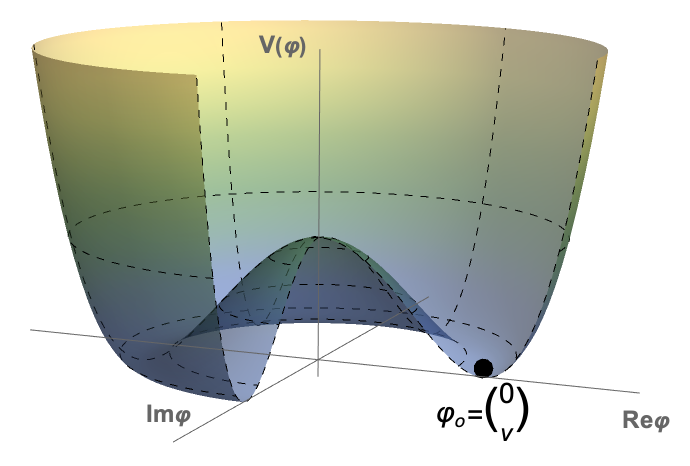
\includegraphics[width=7cm, height=5cm]{mexhat.png}
    \caption{\textit{Η συνάρτηση δυναμικού του μιδαδικού πεδίου $\phi$.}}
    \label{fig:mexhat}
\end{figure}
Για παραχθούν όροι μάζας για τα μποζόνια βαθμίδας 
%με μάζα. Αυτή η ανεπάρκεια επικρατεί γενικά στις τοπικές %θεωρίες βαθμίδας και θεραπεύεται με την 
εισάγουμε ένα βαθμωτό πεδίο, $\phi$, στη βασική αναπαράσταση της ομάδας $SU(2)$ - το πεδίο Higgs. Οι τέσσερις βαθμοί ελευθερίας (β.ε.) του πεδίου $\phi$ 
\begin{equation}\label{scalar SU doublet}
    \phi\,=\,\left(\begin{array}{c} \phi\superscr{+}\\ \phi\superscr{0} \end{array}\right), \qquad\phi\superscr{0},\phi\superscr{+}\in\mathbb{C}
\end{equation}
μετασχηματίζονται σύμφωνα με την \eqref{electroweak transformation}.
Η συνάρτηση δυναμικού του πεδίου πρέπει να ικανοποιεί τις ιδιότητες της επανακανονικοποίησης και να σέβεται τις συμμετρίες ως προς τους $SU(2)\subscr{L}\times U(1)\subscr{Y}$ μετασχηματισμούς. Η πιο γενική Λαγκραντζιανή 
%συνάρτηση βαθμωτού πεδίου που ικανοποιεί τα προαναφερόμενα 
είναι
\begin{equation}\label{scalar boson lagragian}
    \mathcal{L}\subscr{\phi}\,=\,|D\subscr{\mu}\phi|\superscr{2}-V(\phi)\,=\,|D\subscr{\mu}\phi|\superscr{2}+\mu\superscr{2}\phi\superscr{\dagger}\phi - \lambda(\phi\superscr{\dagger}\phi)\superscr{2}
\end{equation}
Όταν οι δύο παραμέτροι $\mu\superscr{2},\lambda\in\mathbb{R}$ ειναι θετικές, το δυναμικό ελαχιστοποιείται από ένα σύνολο εκφυλισμένων καταστάσεων για τις οποίες ισχύει
\begin{equation}
\begin{split}
    &|\phi|\superscr{2}=v\superscr{2},\quad v\in \mathbb{R}\\
    &\min V(\phi\superscr{\dagger}\phi)=V(v\superscr{2})
\end{split}
\end{equation}
\\

Εάν $\left|\Omega\right>$ είναι μια κατάσταση κενού, στην οποία η αναμενόμενη τιμή του πεδιακού τελεστή $\phi$ είναι μη μηδενική, $\left<\Omega\right|{\phi}\left|\Omega\right>\ne 0$, 
τότε αυτή πρέπει να μετασχηματίζεται κάτω από τη δράση της μοναδιακού τελεστή $U(g)$ (όπου $g\in SU(2)\subscr{L}\times U(1)\subscr{Y}$), στην ορθοκανονική κατάσταση $\left|\Omega'\right>\equiv U\left|\Omega\right>$, με την ίδια ενέργεια αλλά διαφορετική αναμενόμενη τιμή για τον πεδιακό τελεστή $\phi$: 
\begin{equation}\label{vacuum exp value symmetry group action}
    \left<\Omega'\right|{\phi}\left|\Omega'\right> = e\superscr{i\alpha\superscr{i}\frac{\sigma\superscr{i}}{2}}e\superscr{i\beta Y}\left<\Omega\right|{\phi}\left|\Omega\right>
\end{equation}
Από τη συζήτηση της ενότητας \ref{spontaneous symmetry breaking} αναμένουμε ότι η πραγματική κατάσταση κενού θα είναι 
%συμμετρική αλλά θα επιλεγεί 
μια από τις εκφυλισμένες καταστάσεις $\left|\Omega\right>$, με μη μηδενική αναμενόμενη τιμή $\left<\phi\right>$. 
%Έχοντας περιοριστεί σε μια συγκεκριμένη κατάσταση, το πεδίο %απαγορεύεται να "μεταβεί" σε κάποια άλλη από το εκφυλισμένο %σύνολο. Μια τέτοια μετάβαση αντιστοιχεί στη δράση της ομάδας %συμμετρίας ή κάποιου υποσυνόλου. Επομένως, η απαγόρευση %μετάβασης
Ως αποτέλεσμα οι β.ε. της διπλέτας που περιγράφουν το κενό δεσμεύονται και κάποια από τα σωματίδια βαθμίδας αποκτούν μάζα. %Οποιαδίποτε διπλέτα γράφεται ως η δράση στοιχείων της ομάδας %συμμετρίας στη γενική διπλέτα \eqref{scalar SU doublet} και το %αντίστροφο. 
Μια γενική διπλέτα παράγεται από μια $SU(2)$ περιστροφή συγκεκριμένης διπλέτας με $\phi\superscr{+}=0$ και $\phi\superscr{0}\in\mathbb{C}$
\begin{equation}\label{scalar doublet with zero comp and su2 tran}
    \phi\,=\,e\superscr{i\xi\superscr{i}\frac{\sigma\superscr{i}}{2}}\left(\begin{array}{c} 0\\ \phi\superscr{0} \end{array}\right)
\end{equation}
Η 
%δράση με την αντίστροφη 
περιστροφή αφήνει την $\mathcal{L}\subscr{\phi}$ αναλλοίωτη και καθιστά μια γενική διπλέτα \eqref{scalar SU doublet} ισοδύναμη %(όσον αφορά την $\mathcal{L}\subscr{\phi}$) 
με την 
%απλούστερη 
\begin{equation}\label{scalar doublet with zero comp}
    \Bar{\phi}\subscr{0}\,=\,\left(\begin{array}{c} 0\\ \phi\superscr{0} \end{array}\right)
\end{equation}
Με βάση τη 
%χρήση της 
διπλέτα \eqref{scalar doublet with zero comp}, "δεσμεύονται" δύο από τους τέσσερις β.ε. του πεδίου Higgs \cite{itzykson2012quantum}. 
%Αυτή η περιστροφή είναι, η ίδια, ένας μετασχηματισμός βαθμίδας %και ακολουθείται από απαραίτητους μετασχηματισμούς σε δυναμικά %βαθμίδας και άλλα πεδία που συνοψίζονται στο . 
Για να βρούμε το ελάχιστο του δυναμικού, βρίσκεται αντικαθιστούμε για $\Bar{\phi}\subscr{0}$ στο δυναμικό, $V(\phi\superscr{\dagger}\phi)$, και ελαχιστοποιούμε
%με διερεύνηση των ακρότατων 
ως προς $x\equiv|\phi\superscr{o}|\superscr{2}$. Έτσι, βρίσκουμε ένα σύνολο ελαχίστων για διάφορες τιμές του πραγματικού και φανταστικού μέρους της συνιστώσας $\phi\superscr{0}$ με μέτρο
\begin{equation}           v\superscr{2}\equiv\phi\superscr{0\,*}\phi\superscr{0}=(\operatorname{Re}\phi\superscr{0})\superscr{2}+(\operatorname{Im}\phi\superscr{0})\superscr{2}=\frac{\mu\superscr{2}}{2\lambda}
\end{equation}
Το σύνολο των τιμών αυτών αντιστοιχεί στην κυκλική βάση του δυναμικού της γραφικής παράστασης \ref{fig:mexhat}.\\

%Επαναλαμβάνοντας τα προηγούμενα βήματα, 
Η \eqref{scalar doublet with zero comp} παράγεται από έναν $SU(2)\times U(1)$ μετασχηματισμό μιας διπλέτας με μια μόνο πραγματική συνιστώσα
\begin{equation}\label{real scalar doublet and u1 tran}
    \Bar{\phi}\subscr{0}=e\superscr{i\alpha (x)}\left(\begin{array}{c} 0\\ v \end{array}\right),\qquad v=\sqrt{\frac{\mu\superscr{2}}{2\lambda}}
\end{equation}
%Είναι αρκετό να χρησιμοποιηθεί η διπλέτα στα δεξιά της %\eqref{real scalar doublet and u1 tran} εκτελώντας τον %αντίστροφο μετασχηματισμό και 
Δευσμεύοντας λοιπόν ακόμη έναν από τους τέσσερεις β.ε. του πεδίου Higgs, αρκεί να χρησιμοποιήσουμε τη διπλέτα
\begin{equation}\label{real scalar doublet}
     \phi\subscr{0}=\left(\begin{array}{c} 0\\ v \end{array}\right)
\end{equation}
Οι τέσσερις συνολικά γεννήτορες της ομάδας $SU(2)\subscr{L}\times U(1)\subscr{Y}$ 
%(τρεις της SU(2) και ένας από U(1)) 
αντιστοιχούν με τους τέσσερις β.ε. του πεδίου Higgs \eqref{scalar SU doublet}. Η \eqref{real scalar doublet} αντιστοιχεί στη μαύρη κουκίδα της εικόνας \ref{fig:mexhat}. Τρεις ανεξάρτητες συμμετρίες σπάζουν, αλλά παραμένει μια που αφήνει την  \eqref{real scalar doublet} αναλλοίωτη. Συνδυάζοντας το γεννήτορα $\frac{\sigma\superscr{3}}{2}$ της $SU(2)$ με τον γεννήτορα $Y$ της $U(1)$, παίρνουμε
\begin{equation}
\left(\begin{array}{cc}
     1 & 0 \\
     0 & 0
\end{array}\right) \phi\subscr{0} = 0
\end{equation}
έχοντας θέσει το υπερφορτίο του $\phi$ ίσο με $\y=\frac{1}{2}$, έτσι ώστε $Y=\frac{\sigma\superscr{0}}{2}$. Έτσι, βρίσκουμε το υποσύνολο των μετασχηματισμών που δεν σπάζουν και αφήνουν την  $\phi\subscr{0}$ αναλλοίωτη:
\begin{equation}
    \phi\subscr{0}\rightarrow e\superscr{i f(x)\,{Q}}\,\phi\subscr{0}=\phi\subscr{0}
\end{equation}
Οι πιο πάνω μετασχηματισμοί σχηματίζουν μια ομάδα $U(1)$ με γεννήτορα τον $Q$
\begin{equation}\label{electric charge quantum number}
    Q\equiv\frac{\sigma\superscr{3}}{2}+Y
\end{equation}
%- αργότερα θα ταυτιστεί με τον κβαντικό αριθμό ηλεκτρικού %φορτίου. Εν τέλη, η κατάσταση του κενού έχει καταλήξει με μια %μόνο (από τις τέσσερεις) πραγματική παράμετρο και παράλληλα ένα %υποσύνολο μετασχηματισμών που την αφήνει αμετάβλητη. 
Οι τρεις β.ε. του πεδίου Higgs που έχουν "δευσμευτεί" απορροφούνται από τα τρία μποζόντια των σπασμένων συμμετριών βαθμίδος παράγοντας τρία διανυσματικά πεδία με μη μηδενική μάζα. %μεταδότες των ασθενών ρευμάτων που αποκτούν μάζα. 

\section{Μάζες μποζονίων βαθμίδας}
Ακολουθούμε την ανάλυση 
%μαθηματική παραγωγή των μαζών 
του Peskin \cite{Peskin:1995ev} και εξετάζουμε τον κινητικό όρο του μποζονικού πεδίου Higgs. Η συναλλοίωτη παράγωγος είναι 
%που εμπεριέχονται στις συναλλοίωτες μερικές παραγώγους $|D\subscr{\mu}\phi|\superscr{2}$ 
\begin{equation}\label{covariant derivative electroweak theory}
    D\subscr{\mu}\equiv\partial\subscr{\mu}-igW\superscr{i}\subscr{\mu}\tau\superscr{i}-ig\subscr{\text{y}}B\subscr{\mu}Y\qquad\tau\superscr{i}\equiv\frac{\sigma\superscr{i}}{2}
\end{equation}
Δρώντας στην κατάσταση $\phi\subscr{0}$, η οποία είναι ομογενής, οι μερικές παράγωγοι μηδενίζονται και έτσι παίρνουμε
\begin{equation}
\begin{split}
    |D\subscr{\mu}\phi\subscr{0}|\superscr{2}\,&=\,\phi\subscr{0}\superscr{\dagger}\,\,(gW\superscr{i}\subscr{\mu}\frac{\sigma\superscr{i}}{2}+g\subscr{\y}B\subscr{\mu}Y)\superscr{2}\,\,\phi\subscr{0}\\
    &=\,\phi\subscr{0}\superscr{\dagger}\,\,(\frac{g}{4}W\superscr{2}\mathbf{1}+gg\subscr{\y}W\superscr{3}\sigma\superscr{3}Y+(g\subscr{\y}BY)\superscr{2})\,\,\phi\subscr{0}
\end{split}
\end{equation}
Με βάση τη \eqref{real scalar doublet} και το υπερφορτίο του $\phi$, βρίσκουμε
\begin{equation}
    |D\subscr{\mu}\phi\subscr{0}|\superscr{2}\,=\,\frac{1}{4}v\superscr{2}g\superscr{2}W\superscr{2}-\frac{1}{2}v\superscr{2}gg\subscr{\y}W\superscr{3}B+\frac{1}{4}(vg\subscr{\y})\superscr{2}B\superscr{2}
\end{equation}
Καταλήγουμε σε τρεις όρους με μάζας, 
οι οποίοι 
%τρεις όροι 
γράφονται στην 
%πιο οικεία 
μορφή γινομένου πινάκων 
%που θυμίζει όρο μάζας
\begin{equation}
    |D\subscr{\mu}\phi\subscr{0}|\superscr{2}\,=\,\frac{1}{2}\,(m\superscr{2})\superscr{ab}\Gamma\superscr{a}\subscr{\mu}\Gamma\superscr{b\,\mu}
\end{equation}
όπου
%με τους δείχτες a,b να προσδιορίζουν τα στοιχεία της τετραπλέτας των μποζονικών πεδίων 
\begin{equation}\label{A quadraplet}
    \Gamma\subscr{\mu}\equiv (W\superscr{1}\subscr{\mu}, W\superscr{2}\subscr{\mu}, W\superscr{3}\subscr{\mu}, B\subscr{\mu})
\end{equation}
και $m\superscr{2}$ ο πίνακας μάζας
\begin{equation}
    m\superscr{2}\equiv\frac{v\superscr{2}}{2}\left(\begin{array}{cccc}
        g^2 & 0 & 0 & 0 \\
        0 & g^2 & 0 & 0 \\
        0 & 0 & g^2 & -gg\subscr{\y} \\
        0 & 0 & -gg\subscr{\y} & g\subscr{\y}^2
    \end{array}\right)
 \end{equation}
Ο πίνακας μάζας όμως δεν είναι διαγώνιος για την εξαγωγή των μαζών των φυσικών σωματιδίων. Διαγωνοποιούμε τον πίνακα μάζας $m\subscr{D}\superscr{2}$ με τον ακόλουθο μετασχηματισμό ομοιότητας 
%του $m\superscr{2}$
\begin{equation}\label{diagonal mass matrix}
    m\superscr{2}\subscr{D}\,=\,E\superscr{-1}\,m\superscr{2}\,E\,=\,\frac{v\superscr{2}}{2}\,\cdot\,\text{diag}\left(g\superscr{2}\,,\,g\superscr{2}\,,\,(g\superscr{2}+g\subscr{\y}\superscr{2})\,,\,0\right)
\end{equation}
όπου 
%οι στήλες του πίνακα Ε είναι τα ιδιοδιανύσματα του %$m\superscr{2}$ (εκφρασμένα ως γραμμικοί συνδυασμοί των %στοιχείων της τετραπλέτας \eqref{A quadraplet})
\begin{equation}
    E \,=\, \left( \begin{array}{cccc}
         1 & 0 & 0 & 0 \\
         0 & 1 & 0 & 0 \\
         0 & 0 & \frac{g}{\sqrt{g\superscr{2}+g\subscr{\y}\superscr{2}}} & \frac{g\subscr{\y}}{\sqrt{g\superscr{2}+g\subscr{\y}\superscr{2}}}\\
         0 & 0 & \frac{-g\subscr{\y}}{\sqrt{g\superscr{2}+g\subscr{\y}\superscr{2}}} & \frac{g}{\sqrt{g\superscr{2}+g\subscr{\y}\superscr{2}}}
    \end{array} \right)
\end{equation}
Ο μετασχηματισμός ομοιότητας οδηγεί στην νέα βάση μποζονίων βαθμίδας, ως εξής 
%που αποτελείται από τα στοιχεία της τετραπλέτας $W'$
\begin{equation}
    W\subscr{\mu}'\equiv (W\superscr{1}\subscr{\mu},W\superscr{2}\subscr{\mu},Z\superscr{0}\subscr{\mu},A\subscr{\mu}) = (E\superscr{-1})\superscr{ab}\Gamma\superscr{b}\subscr{\mu}
\end{equation}
Τα πεδία $W\superscr{3}$ και $B$ της αρχικής βάσης περιστρέφονται 
%εντός του δυσδιάστατου αυθαίρετου χώρου που ορίζουν, 
στα πεδία $Z\superscr{0}$ και $A$. Το πρώτο, με μάζα $\frac{v}{\sqrt{2}}\sqrt{g\superscr{2}+g\subscr{\y}\superscr{2}}$, αντιστοιχεί στο συνδυασμό
\begin{equation}\label{Z boson}
    Z\subscr{\mu}\superscr{0}\,:=\,\frac{gW\subscr{\mu}\superscr{3}-g\subscr{\y}B\subscr{\mu}}{\sqrt{g\superscr{2}+g\subscr{\y}\superscr{2}}}
\end{equation}
και είναι συζευγμένο με τα ουδέτερα ρεύματα των ασθενών αλληλεπιδράσεων.
Το δεύτερο, με μηδενική μάζα, είναι ο φορέας των ηλεκτρομαγνητικών αλληλεπιδράσεων, το φωτόνιο
\begin{equation}\label{A boson}
    A\subscr{\mu}\,:=\,\frac{g\subscr{\y}W\superscr{3}\subscr{\mu}+gB\subscr{\mu}}{\sqrt{g\superscr{2}+g\subscr{\y}\superscr{2}}}
\end{equation}
Τα πεδία $W\superscr{1}$ και $W\superscr{2}$ αποκτούν μάζα $\frac{vg}{\sqrt{2}}$, και αποτελούν τους ηλεκτρικά φορτισμένους φορείς των ασθενών αλληλεπιδράσεων
\begin{equation}
    W\superscr{\pm}\subscr{\mu}\equiv \frac{1}{\sqrt{2}}(W\superscr{1}\subscr{\mu}\mp iW\superscr{2}\subscr{\mu})
\end{equation}
Συνδέονται με τους αντίστοιχους συνδυασμούς των γεννητόρων $\tau\superscr{1}$ και $\tau\superscr{2}$
\begin{equation}
    \tau\superscr{\pm}\equiv \tau\superscr{1}\pm i\tau\superscr{2}
\end{equation}
Ο ορθογώνιος πίνακας $\Bar{E}\superscr{-1}$ που παράγει την  περιστροφή
\begin{equation}
\left(\begin{array}{c}Z\superscr{0}\\A\end{array}\right)=\underbrace{\frac{1}{\sqrt{g\superscr{2}+g\subscr{\y}\superscr{2}}}\left(\begin{array}{cc}
    g & -g\subscr{\y} \\
    g\subscr{\y} & g
\end{array}\right)}_{\Bar{E}\superscr{-1}}\left(\begin{array}{c}W\superscr{3}\\B\end{array}\right)
\end{equation}
μπορεί να εκφραστεί ως πίνακας περιστροφής στο επίπεδο, συναρτήσει της γωνίας $\theta\subscr{w}$ 
\begin{equation}
\Bar{E}\superscr{-1}\equiv\left(\begin{array}{cc}
    \cos\theta\subscr{w} & -\sin\theta\subscr{w} \\
    \sin\theta\subscr{w} & \cos\theta\subscr{w}
\end{array}\right)
\end{equation}
η οποία ονομάζεται η ασθενής γωνία πρόσμιξης.
Ο λόγος των σταθερών σύζευξης ισούται με την εφαπτομένη της γωνίας πρόσμιξης 
\begin{equation}
    \tan\theta\subscr{w}\,\equiv\,\frac{g\subscr{\y}}{g}
\end{equation}
Επομένως μπορούμε να υπολογίσουμε τη γωνία $\theta\subscr{w}$ με βάση τον λόγο των μαζών των σωματιδίων $W$ και $Z$ 
\begin{equation}
    \theta\subscr{w}\,=\,\cos\superscr{-1}\frac{m\subscr{W}}{m\subscr{Z}}\sim 28^{\circ}
\end{equation}
\\

Τέλος, στη νέα βάση, η συναλλοίωτη παράγωγος \eqref{covariant derivative electroweak theory} γράφεται ως
%συναρτήσει των ιδιοπεδίων \eqref{Z boson} και \eqref{A boson}
\begin{equation}\label{covariant derivative with eigenstates}
    D\subscr{\mu}\equiv \partial\subscr{\mu}-i\frac{g}{\sqrt{2}}(W\superscr{+}\subscr{\mu}\tau\superscr{+}+W\superscr{-}\subscr{\mu}\tau\superscr{-})-i\frac{g}{\cos\theta\subscr{w}}Z\superscr{0}\subscr{\mu}(\tau\superscr{3}-\sin\superscr{2}\theta\subscr{w}Q)-ieA\subscr{\mu}Q
\end{equation}
Έχοντας ταυτίσει το πεδίο $A\subscr{\mu}$ με το φωτόνιο, βρίσκουμε τη σταθερά σύζευξη του με φορτισμένα πεδία
\begin{equation}
    e \equiv \frac{gg\subscr{\y}}{\sqrt{g\superscr{2}+g\subscr{\y}\superscr{2}}}=g\sin\theta\subscr{w}
\end{equation}
Το ηλεκτρικό φορτίο ταυτίζεται με την ιδιοτιμή του γεννήτορα $Q$: 
%με τον κβαντικό αριθμό ηλεκτρικού φορτίου
\begin{equation}
    Q=\tau\superscr{3}+Y
\end{equation}
%Η μορφή του Q είναι όπως και στην \eqref{electric charge %quantum number} με τη διαφορά ότι το υπερφορτίο %$Y=\y\sigma\superscr{o}$ καθορίζεται ανάλογα με την SU(2) %αναπαράσταση και το ηλεκτρικό φορτίο του πεδίου στο οποίο δρα ο %τελεστής \eqref{covariant derivative with eigenstates}. 
Η λαγκραντζιανή της ηλεκτρασθενούς θεωρίας, στη βαθμίδα όπου το Higgs δίδεται από την πραγματική διπλέτα που παρουσιάσαμε πιο πάνω, και αγνοώντας τους φερμιονικούς όρους, δίδεται συναρτήσει των φυσικών πεδίων $A\subscr{\mu},Z\subscr{\mu}$, $W\subscr{\mu}\equiv W\subscr{\mu}\superscr{+}$, $W^{\dagger}\subscr{\mu}\equiv W\subscr{\mu}\superscr{-}$
\begin{equation}\label{electroweak lagragian in terms of physical fields}
\begin{split}
    \mathcal{L}=& -\frac{1}{2}|\overline{D}\subscr{\mu}W\subscr{\nu}-\overline{D}\subscr{\nu}W\subscr{\mu}|\superscr{2}\,\,-\,\,\frac{1}{4}F\subscr{\mu\nu}\superscr{2}\,\,-\,\,\frac{1}{4}Z\subscr{\mu\nu}\superscr{2}\,\,+\,\,(\partial\subscr{\mu}\phi)\superscr{2}\\
    & +\frac{1}{2}g\superscr{2}\phi\superscr{2}|W\subscr{\mu}|\superscr{2}\,\,+\,\,\frac{1}{2}\frac{g\superscr{2}\phi\superscr{2}}{2\cos\superscr{2}\theta\subscr{w}}Z\subscr{\mu}\superscr{2}\\
    & -ig\left(\sin\theta\subscr{w}F\subscr{\mu\nu}+\cos\theta\subscr{w}Z\subscr{\mu\nu}\right)W\superscr{\dagger\,\mu}W\superscr{\nu}\\
    & +\frac{1}{2}g\superscr{2}\left( (W\subscr{\mu}\superscr{\dagger}W\subscr{\nu})\superscr{2}-(W\superscr{\dagger}\subscr{\mu}W\superscr{\mu})\superscr{2} \right)\\
    &-\lambda(\phi\superscr{2}-v\superscr{2})\superscr{2}
\end{split}
\end{equation}
Η συναλλοίωτη παράγωγος των μποζονίων W είναι η ακόλουθη
\begin{equation*}
    \overline{D}\subscr{\mu}\equiv\partial\subscr{\mu}-ig(\cos\theta\subscr{w}Z\subscr{\mu}+\sin\theta\subscr{w}A\subscr{\mu})
\end{equation*}
Η αρχική συμμετρία είναι σπασμένη στην $U(1)$ συμμετρία του ηλεκτρομαγνητισμού.

\section{Φερμιόνια στο καθιερωμένο Πρότυπο}
Η αυθόρμητη ρήξη της συμμετρίας από το πεδίο Higgs επιτρέπει την εισαγωγή φερμιονικών όρων μάζας. 
%ενώ ήταν αρχικά αδύνατο να συμπεριληφθούν ρητά στην %Λαγκρατζιανή. 
Σε αντίθεση με το καθιερωμένο πρότυπο, η θεωρία Dirac για ένα σχετικιστικό φερμιονικό πεδίο επιδέχεται άμεσα όρους μάζας, καθώς η απαίτηση για αναλλοιώτητα κατά Lorentz ικανοποιείται εύκολα
\begin{equation}\label{Dirac lagragian}
    \mathcal{L}\subscr{D}=\Bar{\psi}(i\slashed{\partial}-m)\psi
\end{equation}
Οι σπίνορες $\psi$ του Dirac γράφονται συναρτήσει ενός αριστερόστροφου $\psi\subscr{L}$ και δεξιόστροφου $\psi\subscr{R}$ σπίνορα ως εξής
\begin{equation}
    \psi\,=\, \left( \frac{1-\gamma\superscr{5}}{2} \right)\psi+\left( \frac{1+\gamma\superscr{5}}{2} \right)\psi \equiv \psi\subscr{L}+\psi\subscr{R}
\end{equation}
Αντικαθιστώντας στην \eqref{Dirac lagragian} και χρησιμοποιώντας τις ταυτότητες $\{\gamma\superscr{5},\gamma\superscr{0}\}=0$, $(\gamma\superscr{5})\superscr{2}=1$, $(\gamma\superscr{5})\superscr{\dagger}=\gamma\superscr{5}$, βρίσκουμε ότι οι όροι μάζας με δύο $\psi\subscr{L}$ ή δύο $\psi\subscr{R}$ μηδενίζονται:
\begin{equation}
    m\Bar{\psi}\subscr{L}\psi\subscr{L}=\Bar{\psi}\left( \frac{1+\gamma\superscr{5}}{2} \right)\left( \frac{1-\gamma\superscr{5}}{2}\psi \right) = 0
\end{equation}
%ενώ συμβαίνει το αντίθετο με τους κινητικούς όρους. 
Η αναλλοιότητα ως προς μετασχηματισμούς βαθμίδας στο καθιερωμένο πρότυπο απαγορεύει όρους μάζας με έναν αριστερόστροφο και έναν δεξιόστροφο σπίνορα
\begin{equation}\label{dirac mass terms}
    m\bar{\psi}\subscr{L}\psi\subscr{R}
\end{equation}
\subsection{Χειραλικότητα}
Εξαιτίας της χειραλικότητας των ασθενών αλληλεπιδράσεων 
%είναι η αιτία της διαφοράς μεταξύ των μετασχηματισμών 
μετασχηματίζονται διαφορετικά οι δεξιόστροφοι και οι αριστερόστροφοι σπίνορες ως προς μετασχηματισμούς βαθμίδας. %πεδίων και κατ΄επέκταση έχει καταληκτικές συνέπειες για τους %όρους μάζας. 
Τα δεξιόστροφα φερμιόνια, $\psi\subscr{R}$, δεν αλληλεπιδρούν ασθενώς. Επομένως μετασχηματίζονται σύμφωνα με την τετριμμένη μοναδιαία αναπαράσταση (singlet) της $SU(2)$. Το ηλεκτρικό τους φορτίο ισούται με το υπερφορτίο. Ως προς μετασχηματισμούς 
%της ομάδας 
βαθμίδας, μετασχηματίζονται με μια μιγαδική φάση, ανάλογα με το υπερφορτίο τους 
%που οφείλεται στο U(1) κομμάτι
\begin{equation}
    \psi\subscr{R}\rightarrow e\superscr{i\beta\y}\psi\subscr{R}
\end{equation}
\\

Τα αριστερόστροφα φερμιόνια αλληλεπιδρούν ασθενώς %αλληλεπιδράσεις 
και συνεπώς οι μετασχηματισμοί βαθμίδας εμπλέκουν την ομάδα $SU(2)$.
%παίρνουν διαφορετική μορφή. 
Οι λεπτονικές διεργασίες ασθενών αλληλεπιδράσεων σέβονται αυστηρά την ταξινόμηση σε τρεις λεπτονικές οικογένειες: $e$, $\mu$ και $\tau$ και διατηρούν τους τρεις 
%αντίστοιχους 
λεπτονικούς αριθμούς.
Για παράδειγμα, οι διασπάσεις $\mu\rightarrow e\Bar{\nu}\subscr{e}\nu\subscr{\mu}$ και $e\superscr{-}\rightarrow\nu\subscr{e}W\superscr{-}$ παρατηρούνται πειραματικά, όχι όμως οι διασπάσεις $W\superscr{-}\rightarrow e\nu\subscr{\mu}$, $\mu\rightarrow e\nu\subscr{e}\Bar{\nu}\subscr{\mu}$, $\mu\rightarrow e\gamma$. Οι ασθενείς αλληλεπιδράσεις 
%φαίνεται μόνο να περιστρέφουν 
εμπλέκουν κάθε αριστερόστροφο λεπτόνιο και το αντίστοιχο αριστερόστροφο νετρίνο. 
%και το αντίστροφο.
Έτσι, τα λεπτόνια μετασχηματίζονται στη βασική αναπαράσταση της $SU(2)$ σχηματίζοντας τις διπλέτες
\begin{equation}
    \ell\subscr{L}\superscr{i}\equiv\left(\begin{array}{c} \nu\subscr{i} \\ i \end{array}\right)\subscr{L},\qquad i=e,\mu,\tau
\end{equation}
%με τα στοιχεία κάθε διπλέτας να έχουν τον ίδιο λεπτονικό αριθμό %οικογένειας. 
Παρομοίως τα quarks ταξινομούνται σε τρεις οικογένειες ως ακολούθως
\begin{equation}
    q\subscr{L}\equiv \left(\begin{array}{c} u \\ d \end{array}\right)\subscr{L},\,\left(\begin{array}{c} c \\ s \end{array}\right)\subscr{L},\,\left(\begin{array}{c} t \\ b \end{array}\right)\subscr{L} 
\end{equation}
Σε αντίθεση με την διατήρηση των λεπτονικών αριθμών, 
%στα quarks δεν ισχύει το ανάλογο. Οι 
υπάρχουν ασθενείς διεργασίες 
%έχουν δείξει πειραματικά να 
που εμπλέκουν quarks από διαφορετικές οικογένειες, όπως για παράδειγμα, η διάσπαση $s\rightarrow uW\superscr{-}$ \cite{Griffiths:111880}. \\
%Λεπτομέρειες για αυτή τη συμπεριφορά των ασθενών αλλ. στο %κεφάλαιο 10 του . 

Τα αριστερόστροφα φερμιόνια λοιπόν $\psi\subscr{L}\equiv\ell\superscr{i}\subscr{L},\,q\subscr{i,L}$ μετασχηματίζονται ως ακολούθως
\begin{equation}
    \psi\subscr{L}\rightarrow e\superscr{i\alpha\superscr{i}\frac{\sigma\superscr{i}}{2}}e\superscr{i\beta Y}\psi\subscr{L}
\end{equation}
Επομένως οι όροι μάζς \eqref{dirac mass terms}
%, αν και αναλλοίωτη κατά Lorentz, 
δεν είναι αναλλοίωτοι ως προς τους μετασχηματισμούς βαθμίδας και έτσι δεν μπορούν να εμφανιστούν στην $\mathcal{L}$. \\

Το υπερφορτίο κάθε διπλέτας μπορεί να προσδιοριστεί με βάση 
%τον κβαντικό αριθμό 
το ηλεκτρικό φορτίο Q \eqref{electric charge quantum number}. Για παράδειγμα, οι συνιστώσες της διπλέτας $\ell\superscr{e}\subscr{L}$ έχουν ηλεκτρικά φορτία 0 και -1, αντίστοιχα και έτσι το υπερφορτίο που αντιστοιχεί στη διπλέτα ισούται με $\y=-\frac{1}{2}$. Οι συνιστώσες της διπλέτας των quarkς $q\subscr{u,L}$ έχουν ηλεκτρικά φορτία $\frac{2}{3}$ και $-\frac{1}{3}$ αντίστοιχα, και επομένως το υπερφορτίο ισούται με $\y=+\frac{1}{6}$.


\subsection{Η πλήρης θεωρία \texorpdfstring{$SU(3)\,\times\,SU(2)\,\times\,U(1)$}{TEXT}}
Το καθιερωμένο πρότυπο περιλαμβάνει επίσης την περιγραφή των ισχυρών αλληλεπιδράσεων των quarks. Η περιγραφή βασίζεται σε μια μη αβελιανή θεωρία βαθμίδας με ομάδα την $SU(3)$. Οι ομάδα αυτή έχει οκτώ γεννήτορες και επομένως υπάρχουν οκτώ φορείς για την ισχυρή δύναμη, τα γκλουόνια, που είναι άμαζα σωματίδια με σπιν 1. 
%κατασκευάζει τη μη αβελιανή θεωρία βαθμίδας με τα απορρέοντα %οκτώ (όσα και οι γεννήτορες) άμαζα σπιν-1 μποζόνια στην συζυγή %αναπαράσταση (adjoint representation) να είναι οι μεταδότες των %ισχυρών δυνάμεων - gluons. 
Τα quarks έχουν την ιδιότητα του χρώματος 
%στο πλαίσιο των ισχυρών δυνάμεων διεκδικούν φορτίο, τον %κβαντικό αριθμό χρώματος (color) 
με τρείς τιμές, κόκκινο (r), πράσινο (g) και μπλε (b) και έτσι μετασχηματίζονται με βάση τη θεμελιώδη αναπαράσταση της $SU(3)$ με διαστατικότητα 3. 
%Τα gluons αλληλεπιδρούν με τα quarks αλλάζοντας το χρωματικό %τους φορτίο. 
Σε αυτό το σημείο, 
Τα φερμιόνια της πρώτης οικογένειας μπορούν να ταξινομηθούν με βάση τις $U(1)$, $SU(2)$ και $SU(3)$ αναπαραστάσεις τους - δες πίνακα \ref{tab:table with particles and su3, su2 representations}. 

\begin{table}
    \centering
    \begin{tabular}{|m{0.25cm}|m{4.5cm}|m{2cm}|m{2cm}|m{1.9cm}|m{1.4cm}|}
    \cline{2-6}
    \multicolumn{1}{m{0.25cm}|}{} & \centering \textbf{(3,2,1/6)} & \centering \textbf{(3,1,2/3)} & \centering \textbf{(3,1,-1/3)} & \centering \textbf{(1,2,-1/2)} & \textbf{(1,1,-1)} \\
    \hline
     \rotatebox{90}{SU(2)} & \[ \left(\left(\begin{array}{c}
         u^r \\ \\ d^r
    \end{array}\right)_L,\left(\begin{array}{c}
        u^g \\ \\ d^g
    \end{array}\right)_L, \left(\begin{array}{c}
         u^b \\ \\ d^b 
    \end{array}\right)_L\right)\] & \center{$(u^r,u^g,u^b)\subscr{R}$} & \center{$(d^r,d^g,d^b)\subscr{R}$} & \[\left(\begin{array}{c}
         \nu \\ \\ e
    \end{array}\right)_L\] & $\quad\, e_R$ \\
    \hline
    \multicolumn{1}{c}{} & \multicolumn{5}{|c|}{\textbf{SU(3)}} \\
    \cline{2-6}
    \end{tabular}
    \caption{\textit{Οι αναπαραστάσεις των φερμιονίων ως προς τις ομάδες συμμετρίας του καθιερωμένου προτύπου.}}
    %SU(2) - διαστατικότητας d=2 (διπλέτες) για τα %αριστερόστροφα (L) και d=1 (singlets) για τα δεξιόστροφα %(R). Ταυτόχρονα, οι αναπαραστάσεις ως προς SU(3) - d=3 %(τριπλέτες) για τα quarks και διαστατικότητας 1 (singlets) %για τα λεπτόνια. Το υπερφορτίο Y της U(1) βαθμίδας είναι το %τρίτο στοιχείο στην αρχή κάθε στοίλης, π.χ. 1/6 για τα L %quarks.
    \label{tab:table with particles and su3, su2 representations}
\end{table}

\subsection{Φερμιονικοί όροι μάζας}\label{section mass for fermions}
%Ανίκανοι να χρησιμοποιήσουμε όρους μάζας καταφεύγουμε στην 
Αξιοποιούμε το μηχανισμό Higgs με βάση τον οποίο τα μποζόνια βαθμίδος αποκτούν μάζα. Εισάγουμε στους όρους \eqref{dirac mass terms} το πεδίο $\phi$ με υπερφορτίο $y=1/2$
\begin{equation}
    \Bar{\psi}\subscr{L}\cdot\phi\psi\subscr{R} \,+\, \text{h.c.}
\end{equation}
επιτυγχάνοντας έτσι την αναλλοιότητα ως προς όπλους τους μετασχηματισμούς βαθμίδας. 
%το μηδενισμό του συνολικού υπερφορτίου. 
Για μια λεπτονική διπλέτα μόνο μια από τις δύο συνιστώσες αποκτά μάζα, με το νετρίνο να παραμένει άμαζο. 
%θεωρούνται άμαζα στο καθιερωμένο πρότυπο. 
Συγκεκριμένα, στην περίπτωση της διπλέτας ηλεκτρονίου έχουμε
\begin{equation}
    \lambda\subscr{e}\Bar{\ell}\subscr{L}\superscr{e}\cdot\phi e\subscr{R} + \text{h.c.}
\end{equation}
όπου $\lambda$ μια αδιάστατη σταθερά σύζευξης. Το Higgs σπάζει τη συμμετρία αποκτώντας την αναμενόμενη τιμή \eqref{real scalar doublet}. Έτσι παίρνουμε τον όρο μάζας για το ηλεκτρόνιο
\begin{equation}
    \lambda\subscr{e}v\Bar{e}\subscr{L}e\subscr{R} + \text{h.c.}
\end{equation}
Η μάζα του ηλεκτρονίου είναι ανάλογη της αναμενόμενης τιμής $v$ και της σταθεράς σύζευξης $\lambda$:
\begin{equation}
    m\subscr{e}=\lambda\subscr{e}v
\end{equation}